% Created 2021-03-02 Tue 14:42
% Intended LaTeX compiler: pdflatex
\documentclass[11pt]{article}
\usepackage[utf8]{inputenc}
\usepackage[T1]{fontenc}
\usepackage{graphicx}
\usepackage{grffile}
\usepackage{longtable}
\usepackage{wrapfig}
\usepackage{rotating}
\usepackage[normalem]{ulem}
\usepackage{amsmath}
\usepackage{textcomp}
\usepackage{amssymb}
\usepackage{capt-of}
\usepackage{hyperref}
\author{Devin Michael O'Brien}
\date{\today}
\title{Chess Editor}
\hypersetup{
 pdfauthor={Devin Michael O'Brien},
 pdftitle={Chess Editor},
 pdfkeywords={},
 pdfsubject={},
 pdfcreator={Emacs 27.1 (Org mode 9.3)}, 
 pdflang={English}}
\begin{document}

\maketitle
\tableofcontents

\section{Project Definition}
\label{sec:org83eaefe}
\subsection{Revised}
\label{sec:org83ee185}
Devin's:
Chess is a game that has been played by millions since its
conception. It is a game that has relatively simple rules that make it
which make it a game that has been sort of a standard for testing the
computation abilility of automata. Although they have become advanced
enough where chess is no longer sufficient, we feel it is still a good
start for ones' ability. The goal of this project is to develop a
chess application using the Angular framework and test some concepts
that we are interested in, such as User Authentication with Google
Identity and Implementation of an Open-Source Standard like the
Unified Chess Interface; with an added bonus of trying to wrangle with
an External Web Server with Multiplayer.

\subsection{Original}
\label{sec:org3366cab}
People like Chess and need a way to quickly develop and practice new strategies. I love
Chess!!! Chess Editor will let people play Chess on their PC and set up the board the
way they want to test different strategies, or just play in a different way. It will support
playing against an AI, or playing against another person locally. It will include an account
system to track wins and losses. For the purposes of testing, there will be an undo and
redo button, as well as tools to set up specific board scenarios. It will be programmed in
Typescript and we will use Stockfish for the AI.


\section{Project Requirements}
\label{sec:org10e9d36}
\subsection{Functional}
\label{sec:org69c7430}
\subsubsection{Primary Requirements}
\label{sec:org00f27d8}
The primary requirements of functionality for \textbf{Chess Editor}  include:
\begin{itemize}
\item Ability for the user to play an online game of chess with
another user, or alternatively against \textbf{AI} that will be
provided.
\item Ability for the user to track their \textbf{statistics} of play over
the life of their account; such as:
\begin{itemize}
\item Wins
\item Losses
\item Draws
\end{itemize}
\item Ability for the user to modify the starting layout of the chess
pieces to match the configuration of either a previously ongoing
game or a chess scenario (i.e., a game that started offline).
\end{itemize}
\subsubsection{Secondary Requirements}
\label{sec:org5898cea}
The secondary scope of functionality for Chess Editor include:
\begin{itemize}
\item Ability for the end user to create an account to access features
\item Ability for the end user to login via their Google Account credentials.
\end{itemize}
\subsubsection{Optional Requirements}
\label{sec:org4724383}
\subsection{Usability}
\label{sec:org959cf7b}
\subsubsection{User Interface}
\label{sec:org99a4ed1}
The user interface of the application must not be obtrusive and
needs to be adapted for mobile devices.
\subsubsection{Performance}
\label{sec:org3d88320}
The performance of the application must not interfere with other
processes on the users system.
\subsection{System}
\label{sec:orga37de9e}
\subsubsection{Hardware}
\label{sec:orgc32c366}
\begin{enumerate}
\item Severside
\label{sec:org2bc5f76}
All server-side requirments will be provided by the hosting site: ecowebhosting.co.uk
\item Clientside
\label{sec:org61d5652}
The application will require hardware capable of running a modern web-brower without difficulty.
\end{enumerate}
\subsubsection{Software}
\label{sec:org12fcb68}
\begin{enumerate}
\item Clientside
\label{sec:orgf9dfc96}
The application will require a modern web-browser.
\item Serverside
\label{sec:org0768bb3}
The server will require the database and networking software required of a web server.
\end{enumerate}
\subsubsection{Database\hfill{}\textsc{Verify}}
\label{sec:org23811f2}
This project will have one database which is used to keep track of
on-going games. This is specifically MySQL version 10.4.14.

\subsection{Networking}
\label{sec:org45a4f16}
All project artifacts and interconnectivities are provided by the
hosting server.
\subsection{Security}
\label{sec:org90365fe}
For Google Authentication, we will be leveraging the Google OAuth
2.0 API. The other security requirements are inherently provided by
the hosting server.
\section{Project Specification}
\label{sec:org4bce00f}
\subsection{Focus}
\label{sec:orga784189}
This project has a focus on developing experience with Angular and
with a client-server application. This project will attempt to utilize
open-source projects when it is reasonably possible.

\subsection{Development Environemnt}
\label{sec:org28ad283}
\subsubsection{Libraries}
\label{sec:org58ae02c}
This project will be using the Google Identity API for user Authentication.
\subsubsection{Frameworks}
\label{sec:org6625518}
This project will be developed using the Angular framework (11.1.2)
with TypeScript.
\subsection{Platform}
\label{sec:org7f8c0b0}
This project is going to be web-based application,
\subsection{Genre}
\label{sec:org45b583c}
This project is considered as an online board game.
\section{System Design}
\label{sec:org6453a59}
\subsection{Subsystem Identification}
\label{sec:orga8ea2ee}
We will be leveraging our MySQL database engine to create, update,
read, and delete user information.
Google Identity will also be used to facilitate account creation
with a user's exsisting Google account.
\subsubsection{Chess Gameplay}
\label{sec:org6c26c41}
The MySQL database engine will be used for tracking gameplay
metrics.
The Angular framework will be implemented with TypeScript to
manage the gameplay logic and for validation of chess scenarios.
The Stockfish AI framework will be used to respond to the end
player's movement when playing against the "computer".
\subsubsection{Subsystem Communication}
\label{sec:org69dbfdd}
The player will interact with the Chess UI with their keyboard and
mouse. The player will notice a response from the UI with their
monitor. The system should have proper UI responses indicating a
success/failure of the attempted action.
\subsubsection{Sequence Diagram\hfill{}\textsc{@DeMO}}
\label{sec:org4c77b70}
\begin{center}
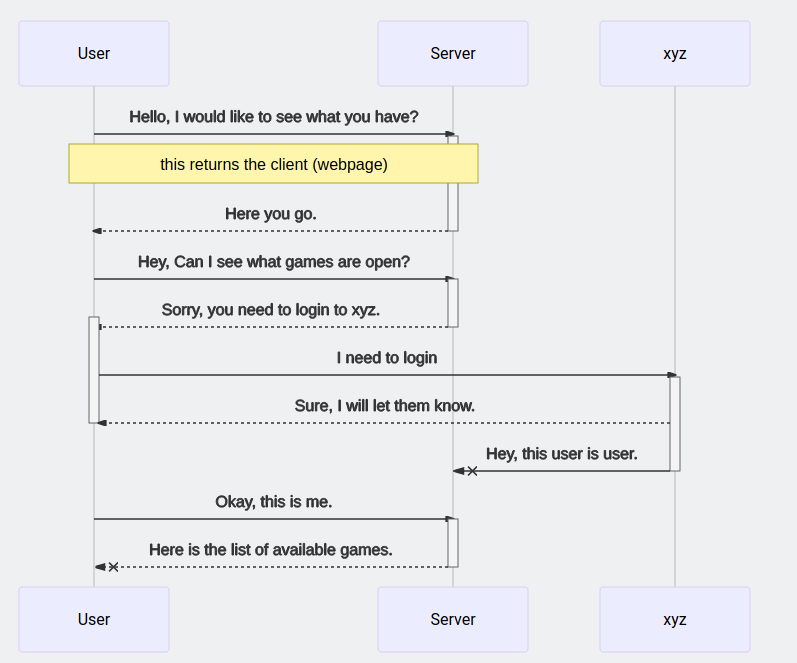
\includegraphics[width=.9\linewidth]{present/Sequence1.png}
\end{center}
\begin{center}
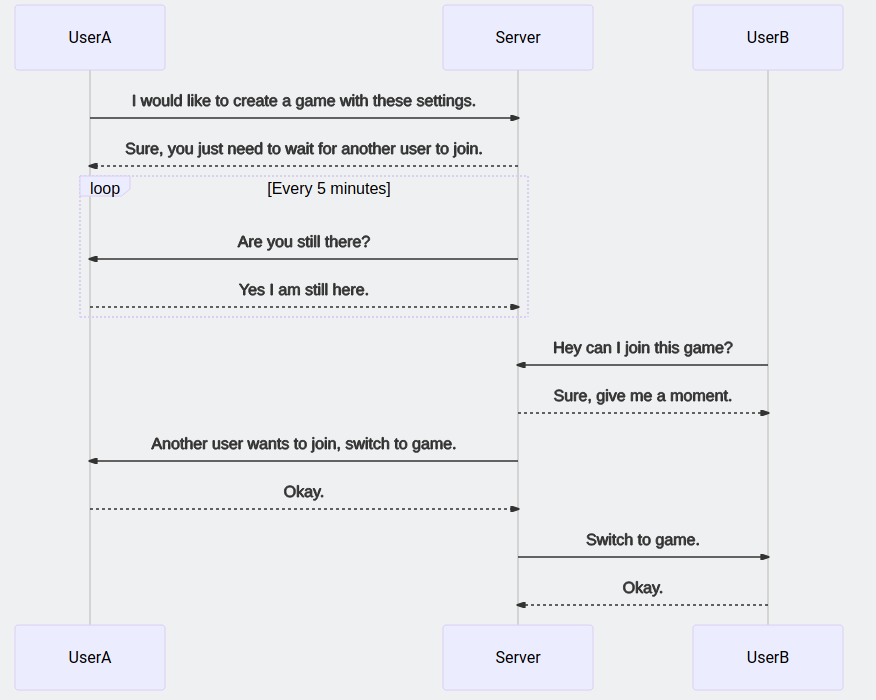
\includegraphics[width=.9\linewidth]{present/Sequence2.png}
\end{center}
\begin{center}
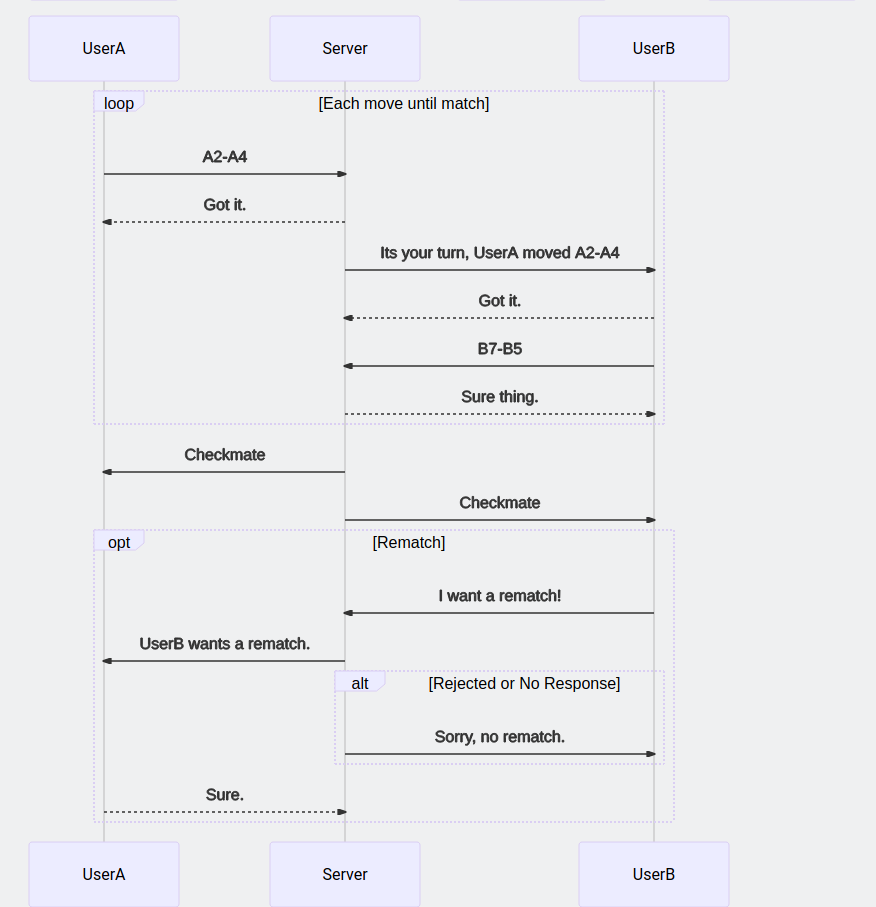
\includegraphics[width=.9\linewidth]{present/Sequence3.png}
\end{center}
\subsubsection{Use-Case Diagram}
\label{sec:org5cf3823}

\subsubsection{Class Diagram\hfill{}\textsc{@Dakota:@Tyler:@DeMO:@pawilliamson}}
\label{sec:orgcba25bc}
\begin{center}
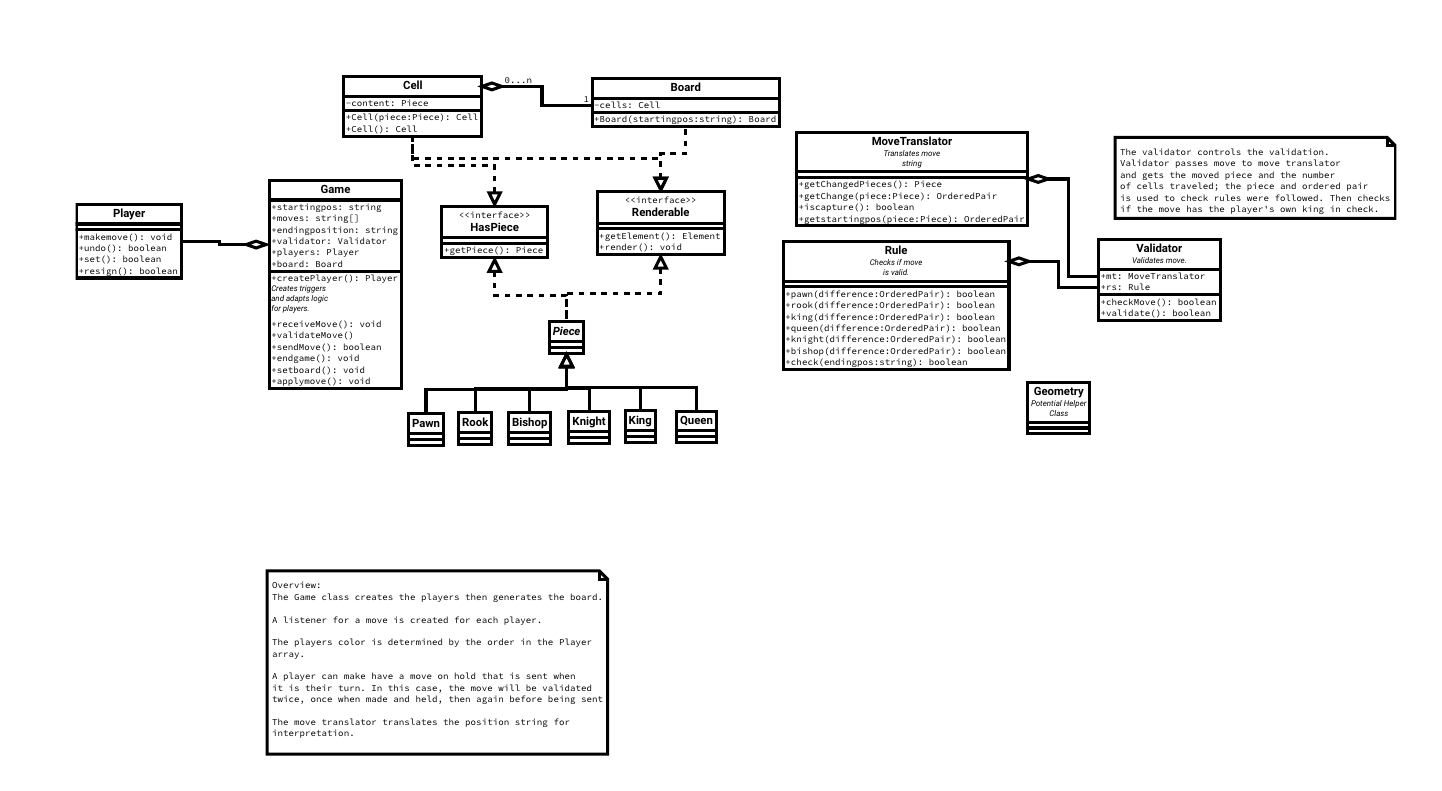
\includegraphics[width=.9\linewidth]{present/ClassDiagram.png}
\end{center}
\subsubsection{Entity Relationship Model (E-R Model)}
\label{sec:org17df613}
\begin{center}
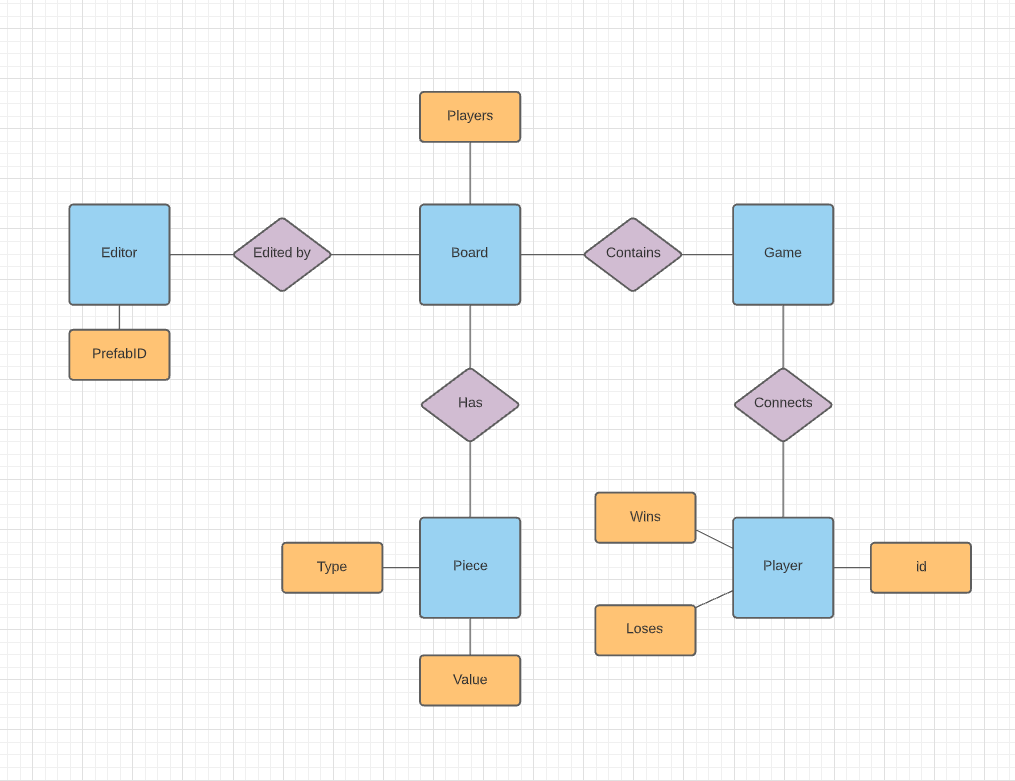
\includegraphics[width=.9\linewidth]{present/ERDiagram.png}
\end{center}
\url{https://lucid.app/lucidchart/b4d167c8-e8fa-475e-9e63-86c4e3aed414/view?page=0\_0\#}
\subsection{Design}
\label{sec:org48665f4}
\subsubsection{Mock-up Diagram}
\label{sec:org84465fd}
\subsubsection{Color Schemes}
\label{sec:orgd5754ee}
\subsubsection{Additional Comments}
\label{sec:org527642e}
We will be using Bootstrap framewwork.
\subsection{Sub-System Communication}
\label{sec:org789c6c4}
\subsubsection{Controls}
\label{sec:org1160952}
\subsubsection{I/O}
\label{sec:org8018958}
\subsubsection{Dataflow\hfill{}\textsc{@Tyler}}
\label{sec:org82fbf72}
\subsection{Entity Relationship Model (E-R Model)}
\label{sec:orgc629d54}
\subsection{Overall operation - System Model$\backslash$}
\label{sec:org791ce30}
\subsubsection{Account Creation Management}
\label{sec:orga6baabb}
The user will modify their account information via the Chess Game
UI that will be fed into their respective records in the database.
\subsubsection{Chess Gameplay Management}
\label{sec:orgb3b815a}
Gameplay metrics will be automatically tracked by the Chess Game
UI in tandem with pre-existing records stored in the MYSQL
database.
Gameplay involvng the "computer" will be handled by the Stockfish
AI program to determine the next best move.
\url{https://lucid.app/lucidchart/invitations/accept/18b1143a-20e9-441c-ac34-2c95f7a2d031}
\section{{\bfseries\sffamily TODO} System Analysis}
\label{sec:org8fe2722}
\subsection{Subsystems}
\label{sec:orgaab7a21}
\begin{itemize}
\item Account Creation/Management
\item Chess Gameplay Management
\end{itemize}
\subsection{System (Tables and Description)}
\label{sec:org4de7c07}
\subsubsection{Data Dictionary}
\label{sec:org4dcca3e}
\begin{center}
\begin{tabular}{llll}
Table & Column & Data Type & Description\\
\hline
User & userID (Pky) & int & UUid of user\\
 & firstName & varchar & User's first name\\
 & lastName & varchar & User's last name\\
 & wins & int & Number of user's wins\\
 & losses & int & Number of user's losses\\
 & activeGameID (fky) & int & UUID of currently active game\\
Game & gameID (Pky) & int & UUID of current game session\\
 & turnList & List<Peice, Integer, Integer> & UUID of recorded turn\\
 & playerOne (fky) & int & UUID of player one (white)\\
 & playerTwo (fky) & int & UUID of player two (black)\\
\end{tabular}
\end{center}
\subsubsection{Process Models}
\label{sec:orgd94a977}
\begin{center}
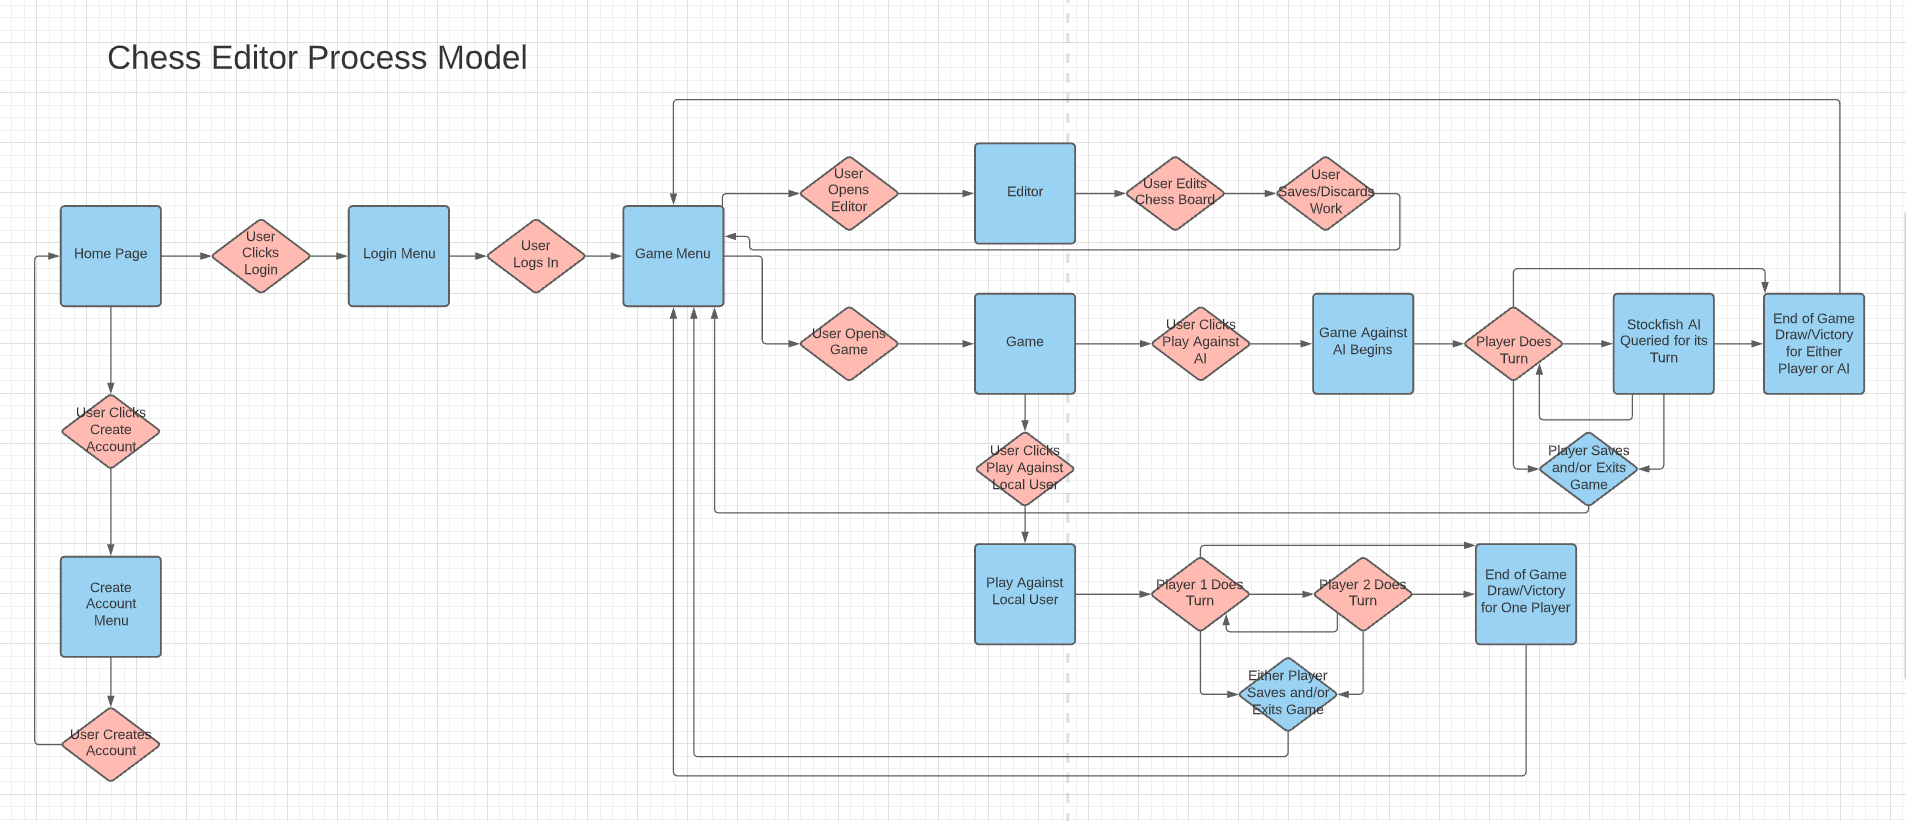
\includegraphics[width=.9\linewidth]{ present/ProcessModel.png}
\end{center}
\url{https://lucid.app/lucidchart/7d69e18e-721a-43ad-a77d-83df4e8d1f3a/view?page=0\_0\#}
\subsection{Algorithm Analysis}
\label{sec:orgf8d9719}
\subsubsection{Big-O Analysis}
\label{sec:orgad44236}
We expect that the game when not playing with an AI will run in
constant time as there is nothing in our current algorithms that
will execute a variable number of times. This will probably change
when the AI is implemented.

\section{{\bfseries\sffamily TODO} Project Scrum Report}
\label{sec:orgaab572c}
\subsection{Overall}
\label{sec:org751c929}
\subsection{Product Backlog}
\label{sec:org3a8e076}
\subsection{Sprint Backlog}
\label{sec:orgca82dbb}
\subsection{Burndown Chart}
\label{sec:org6e38130}
\subsection{Sprint 1}
\label{sec:orgb49d24d}
Sprint 1 began on January 22, 2021 and continued to Febuary
6, 2021. The period lasted one day longer than the allocated duration.
\subsubsection{Scrum}
\label{sec:org27900fe}
During sprint, two scrum meetings took place
\begin{itemize}
\item January 28, 2021: Discussed the framework of the project and
decided to use Angular. Discussed the scope of the project and
decided to be a web application. Discussed authentication
services for the server.
\item February 4, 2021: Discussed some work that was done since the
previous scrum; includes diagrams and investigations of Google
Authentication viability for the server.

\begin{center}
\begin{tabular}{llll}
Item & Created BY & Date & Status\\
Project Definition & dobrienUNCG & 01/21/21 & Completed by pizzaza\\
Project requirements & dobrienUNCG & 01/21/21 & Completed during Scrums 1 and 2 by group\\
Identify subsystems & dobrienUNCG & 01/21/21 & Moved to Sprint 2 backlog\\
Project Specification & dobrienUNCG & 01/21/21 & Moved to sprint 2 backlog\\
\end{tabular}
\end{center}
\end{itemize}

\section{{\bfseries\sffamily TODO} Subsystems [/]}
\label{sec:orgd82a615}
\subsection{{\bfseries\sffamily TODO} Chess Game [0/7]\hfill{}\textsc{@Tyler:@Dakota}}
\label{sec:orgafad8d8}
\subsubsection{{\bfseries\sffamily TODO} Initial Design and Model}
\label{sec:org3e109c5}
\subsubsection{{\bfseries\sffamily TODO} Data Dictionary}
\label{sec:org4167410}
\subsubsection{{\bfseries\sffamily TODO} Revisions (Refinement)}
\label{sec:org753da99}
\subsubsection{{\bfseries\sffamily TODO} Scrum Backlog}
\label{sec:orgf5bf6e3}
\begin{center}
\begin{tabular}{llll}
Task & On & Assigned To & Completed On\\
--------------------------- & -- & ------------ & -----------\\
Generate Chessboard &  & Tyler, Dakota & \\
Chess Pieces &  &  & \\
Movement &  &  & \\
Movement and player interfaces &  &  & \\
Display Board &  &  & \\
Drag and move piece` &  &  & \\
Validate Moves &  &  & \\
Detect Check &  &  & \\
Detect Win &  &  & \\
\end{tabular}
\end{center}
\begin{enumerate}
\item {\bfseries\sffamily TODO} User Story Categories\hfill{}\textsc{@DeMO}
\label{sec:org3e75f27}
\end{enumerate}
\subsubsection{{\bfseries\sffamily TODO} Coding}
\label{sec:org25e9354}
\begin{enumerate}
\item Language
\label{sec:orgd2b4c32}
\end{enumerate}
\subsubsection{{\bfseries\sffamily TODO} User Training}
\label{sec:org5c70412}
\subsubsection{{\bfseries\sffamily TODO} Testing}
\label{sec:orgf1cad92}
\subsection{{\bfseries\sffamily TODO} User Authentication [0/7]\hfill{}\textsc{@pawilliamson}}
\label{sec:orge8001e2}
\subsubsection{{\bfseries\sffamily TODO} Initial Design and Model}
\label{sec:org53b235b}
\subsubsection{{\bfseries\sffamily TODO} Data Model}
\label{sec:orgebe788a}
\subsubsection{{\bfseries\sffamily TODO} Refinement}
\label{sec:org4fc9bff}
\subsubsection{{\bfseries\sffamily TODO} Scrum Backlog}
\label{sec:orgf4efbe0}
\begin{enumerate}
\item {\bfseries\sffamily TODO} User Story Categories\hfill{}\textsc{@DeMO}
\label{sec:org2314b80}
\end{enumerate}
\subsubsection{{\bfseries\sffamily TODO} Coding}
\label{sec:orgbd8ae53}
\subsubsection{{\bfseries\sffamily TODO} User Training}
\label{sec:org1856922}
\subsubsection{{\bfseries\sffamily TODO} Testing}
\label{sec:org27a128b}
\subsection{{\bfseries\sffamily TODO} Server - Client [0/7]\hfill{}\textsc{@Tyler}}
\label{sec:orgde6549b}
\subsubsection{{\bfseries\sffamily TODO} Initial Design and Model}
\label{sec:org16db1e6}
\subsubsection{{\bfseries\sffamily TODO} Data Dictionary}
\label{sec:orgb1384c9}
\subsubsection{{\bfseries\sffamily TODO} Refinement}
\label{sec:org663730d}
\subsubsection{{\bfseries\sffamily TODO} Scrum Backlog}
\label{sec:orgeb6a832}
\subsubsection{{\bfseries\sffamily TODO} Coding}
\label{sec:org74fc8c2}
\subsubsection{{\bfseries\sffamily TODO} User Training}
\label{sec:orgb966642}
\subsubsection{{\bfseries\sffamily TODO} Testing}
\label{sec:org326e5ec}
\subsection{{\bfseries\sffamily TODO} Computer Opponent  [0/7]\hfill{}\textsc{@DeMO}}
\label{sec:org989699b}
\subsubsection{{\bfseries\sffamily TODO} Initial Design and Model}
\label{sec:org805608e}
\subsubsection{{\bfseries\sffamily TODO} Data Dictionary}
\label{sec:orgb9d9e1e}
\subsubsection{{\bfseries\sffamily TODO} Refinement}
\label{sec:orgf639f6d}
\subsubsection{{\bfseries\sffamily TODO} Scrum Backlog}
\label{sec:orgce14b33}
\begin{enumerate}
\item {\bfseries\sffamily TODO} User Story Categories
\label{sec:org3cb20f3}
\end{enumerate}
\subsubsection{{\bfseries\sffamily TODO} Coding}
\label{sec:org0a4c573}
\subsubsection{{\bfseries\sffamily TODO} User Training}
\label{sec:org6728850}
\subsubsection{{\bfseries\sffamily TODO} Testing}
\label{sec:orgbda6f6b}
\section{{\bfseries\sffamily TODO} Complete System}
\label{sec:org5662fd1}
\subsection{{\bfseries\sffamily TODO} Final Product}
\label{sec:orge13a449}
\subsection{{\bfseries\sffamily TODO} Source code and user manual + Technical Report}
\label{sec:org258ab83}
\subsubsection{{\bfseries\sffamily TODO} GitHub}
\label{sec:org2167192}
\subsection{{\bfseries\sffamily TODO} Evaluation by client and instructor}
\label{sec:org2e92f94}

\subsection{{\bfseries\sffamily TODO} Team Member Description}
\label{sec:org607f4f1}
Our team consists of five members: Dakota Simpkins, Tyler Wallshleger,
Devin O'Brien, Preston Williamson, and Brandon Kyle.
\subsubsection{Dakota Simpkins}
\label{sec:org46555fc}
\subsubsection{Tyler Wallshleger}
\label{sec:orgaa9dcdc}
\subsubsection{Devin O'Brien}
\label{sec:org59815cb}
\subsubsection{Preston Williamson}
\label{sec:org235f7c8}
\subsubsection{Brandon Kyle}
\label{sec:org8530033}
\end{document}
